\section{Architecture}
\subsection{Le système de fichiers}
\begin{frame}
\frametitle{Le système de fichiers}

\begin{block}{Image initial}
\begin{itemize}
\item Busybox
\item Un serveur DHCP
\item Un deamon telnet
\item Un accès au port USB en mode série 
\end{itemize}
\end{block}

\begin{block}{Image final}
\begin{itemize}
\item Un accès au port USB par connexion Ethernet
\item Le support du protocole SSH
\item La librairie DirectFB
\end{itemize}
\end{block}

\end{frame}

\subsection{Driver, ioctl et DirectFB}

\begin{frame}
\frametitle{Driver et ioctl}

\begin{block}{Définition ioctl}
\begin{itemize}
\item Appel système pour des opérations d'entrée/sortie
\item Prend en paramètre un code requête
\end{itemize}
\end{block}
\begin{block}{Les fonctions ioctl du driver permettent :}
\begin{itemize}
\item Mettre à jour l'affichage de l'écran
\item Récupérer des informations relatifs au driver (température, waveform, ...)
\item Modifier des paramètres du driver (température, waveform, ...)
\end{itemize}
\end{block}

\end{frame}

\begin{frame}
\frametitle{DirectFB}

\begin{block}{Intérêts}
\begin{itemize}
\item Ensemble d'API graphiques
\item Interaction directe avec le framebuffer 
\item Aucune modification du kernel
\item Aucune dépendance (sauf libc mais déjà présent)
\end{itemize}
\end{block}

\end{frame}

\begin{frame}
\frametitle{Schéma fonctionnement DirectFB}

\begin{center}
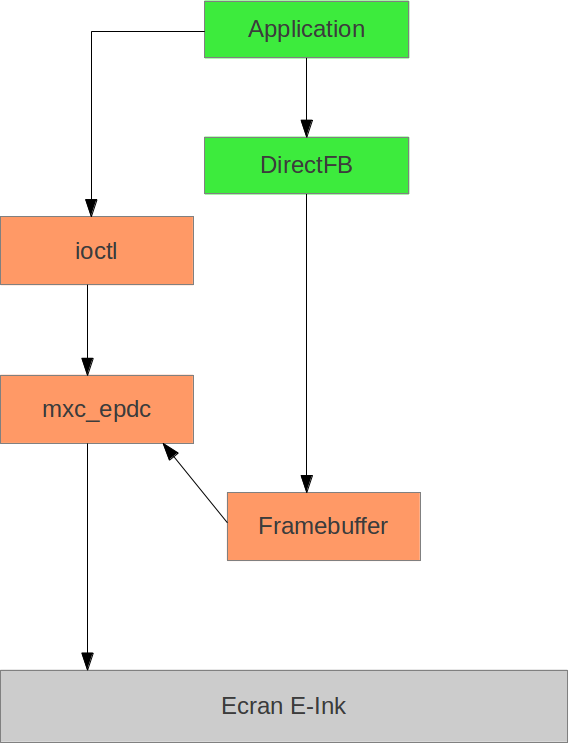
\includegraphics[scale=0.3]{schema_direct_fb.png}
\end{center}

\end{frame}

